\documentclass[parskip=half,DIV=16]{scrartcl}

\title{Project report}
\subtitle{ATM S 544}
\author{Dominik Stiller}
\date{\today}

\usepackage[english]{babel}
\usepackage[utf8]{inputenc}
\usepackage{siunitx,amsmath,physics}
\usepackage{caption,subcaption,graphicx,csquotes,xcolor}
\usepackage{booktabs}
\usepackage{placeins}
\usepackage[
	backend=biber,
	bibwarn=true,
	bibencoding=utf8,
	sortlocale=en_US,
	url=false,
	style=apa,
	isbn=false
]{biblatex}

\definecolor{uw-purple}{RGB}{51, 0, 111}

\usepackage{hyperref}
\hypersetup{
	% hidelinks,
	colorlinks=true,
	linkcolor=black,
	citecolor=black,
	urlcolor=uw-purple
}

\usepackage{doi}
\usepackage{nomencl}
\makenomenclature
\usepackage[noabbrev,capitalise]{cleveref}
\usepackage[acronym,nonumberlist,nopostdot,nogroupskip]{glossaries}
\usepackage[
	outputdir=build,
]{minted}
\setminted{
	linenos,
	tabsize=4,
	fontsize=\small,
}
\newmintinline{python}{}

\usepackage{lmodern}
\usepackage[T1]{fontenc}
\usepackage{inconsolata}
\usepackage{tikz}

\newcommand{\result}[1]{\colorbox{uw-purple}{\textcolor{white}{#1}}}

\setlength{\nomlabelwidth}{1.5cm}
\setlength{\nomitemsep}{-\parsep}
\newcommand{\nomunit}[1]{%
\renewcommand{\nomentryend}{\hspace*{\fill}\si{#1}}}

\sisetup{per-mode=symbol}
\AtBeginDocument{\RenewCommandCopy\qty\SI}

\DeclareGraphicsRule{.ai}{pdf}{.ai}{}

\addbibresource{bibliography.bib}


\makeglossaries
\newacronym{LIM}{LIM}{linear inverse model}
\newacronym{DA}{DA}{data assimilation}
\newacronym{EOF}{EOF}{empirical orthogonal function}
\newacronym{EnSRF}{EnSRF}{ensemble square-root filter}


\begin{document}

\maketitle


\section{Introduction}

For this project, I reproduced some results of \textcite{Perkins2017,Perkins2020,Perkins2021}\footnote{The three Perkins and Hakim papers are hereafter referred to as PH17, PH20, and PH21.}, who reconstructed ten climate fields over the last millennium. Their paleoclimate \gls{DA} method combines the ensemble forecast of a coupled ocean--atmosphere \gls{LIM} with proxy observations by means of an \gls{EnSRF}. Since I will continue this line of research, my project is less concerned with originality and more with familiarizing myself with the data, methods, and workflow. The source code is available at \url{https://github.com/DominikStiller/uw-enspred}.

There are some notable differences of my implementation compared to PH21:
\begin{itemize}
    \item They use training data for the \gls{LIM} from CMIP5 \emph{past1000} simulations, while I use CMIP6 \emph{past2k} experiment data. Therefore, my training dataset is larger and more recent.
    \item Their state vector contains seasonal averages of surface air temperature in addition to annual averages of other fields, while mine only contains annual averages.
    \item They use real proxy observations from the Pages2k, while I generate noisy pseudo-observations from a CMIP6 \emph{past1000} simulation.
    \item They validate against instrumental datasets, while I validate against the simulation from which the pseudo-observations are drawn.
\end{itemize}
Using pseudoproxies and verifying against their true value allows me to check the correctness of my code rather than actually reconstructing the past climate.

My \gls{LIM} training dataset is the \emph{past2k} simulation~\parencite{Jungclaus2017} from coupled ocean--atmosphere models over 1--1849 CE at monthly resolution. The extended simulation compared to the \emph{past1000} experiments allows better investigation of the medieval period; the forcings and spin-up are identical to the shorter variant. For me, the benefit is 850 additional years of training data. I used the \emph{past2k} simulation of the MPI-ESM1-2-LR model, which is the only available one.



\section{Forecasting and data assimilation setup}

\begin{figure}[h]
    \centering
    \includegraphics[width=0.8\textwidth]{figures/architecture.ai}
    \caption{Setup for cycling \gls{DA}.}
    \label{fig:arch}
\end{figure}

The main components of my reconstruction code are shown in \cref{fig:arch}. A mapper translates between the high-dimensional physical space for \gls{DA} and the low-dimensional space for forecasting (\cref{subsec:setup-dimred}). The \gls{LIM} generates an ensemble forecast based on initial conditions in this reduced space (\cref{subsec:setup-lim}). Observations are assimilated in the physical space by the \gls{EnSRF} (\cref{subsec:setup-ensrf}). This section describes the technical aspects of my cycling \gls{DA} setup.


\subsection{Dimensionality reduction for LIM}
\label{subsec:setup-dimred}

The \emph{past2k} simulation output of MPI-ESM1-2-LR contains $\sim$400 fields on its native grid of \qtyproduct{1.875 x 1.875}{\degree}. Like PH21, I regridded the data to a regular \qtyproduct{2.0 x 2.0}{\degree} latitude--longitude grid using bilinear interpolation and selected ten fields: 2 m surface air temperature (TAS), precipitation (PR), sea-level pressure (PSL), 500 hPa geopotential height (ZG500), outgoing top-of-atmosphere longwave radiation (RLUT), reflected top-of-atmosphere shortwave radiation (RSUT), sea-surface temperature (TOS), sea-surface salinity (SOS), dynamic ocean surface height (ZOS), and 0-700 m ocean heat content (OHC700). These are averaged annually from April to March since many real proxies do not have higher temporal resolution. This also means that the \gls{LIM} forecast step is 1 year and the training dataset is reduced to 1849 examples (one year less than 1850 because of the split-year annual average).

The original state vector for each timestep is 162 000-dimensional, even after regridding and field selection, which poses a large computational burden for the \gls{LIM}. PH21 leveraged joint modes of variability to reduce the state to 50 dimensions while retaining sufficient variance. The dimensionality reduction comprises multiple steps:
\begin{enumerate}
    \item Mask out nan values. These do not have to be included in the state vector. For example, ocean fields do not have values over land, and I needed to remove some spurious invalid values, particularly above the poles.
    \item Remove trend. The \gls{LIM} assumes stationary statistics~\parencite{Penland1995} and forecasts anomalies; removing the trend yields these anomalies.
    \item Fit and project each field individually onto \glspl{EOF}. PH21 found that 400 components retain more than 90\% of each field's variance. Each grid cell is latitude-weighted before fitting the \glspl{EOF}.
    \item Standardize each field individually. (The precipitation field is standardized before individual EOF projection since its small magnitude makes it prone to numerical noise.)
    \item Concatenate the 400 individual EOFs of each field except OHC700, then fit and project them onto a joint \gls{EOF}. I retained the leading 30 components, slightly more than PH21 since my data are different. This highlights how coupled field variability really is.
    \item Truncate the OHC700 field to 20 components. This field is kept separate because its dynamics are much slower than the other fields, particularly atmospheric ones.
    \item Concatenate the 30 joint EOF components and the 20 OHC700 components into a single 50-dimensional vector, which forms the reduced state vector.
\end{enumerate}
To map back into physical space, these steps are applied in reverse order. The dimensionality reduction compresses the ten fields from 26 GB down to just 1 MB (a factor 12 of which is due to the annual averaging).

\begin{figure}[h]
    \centering
    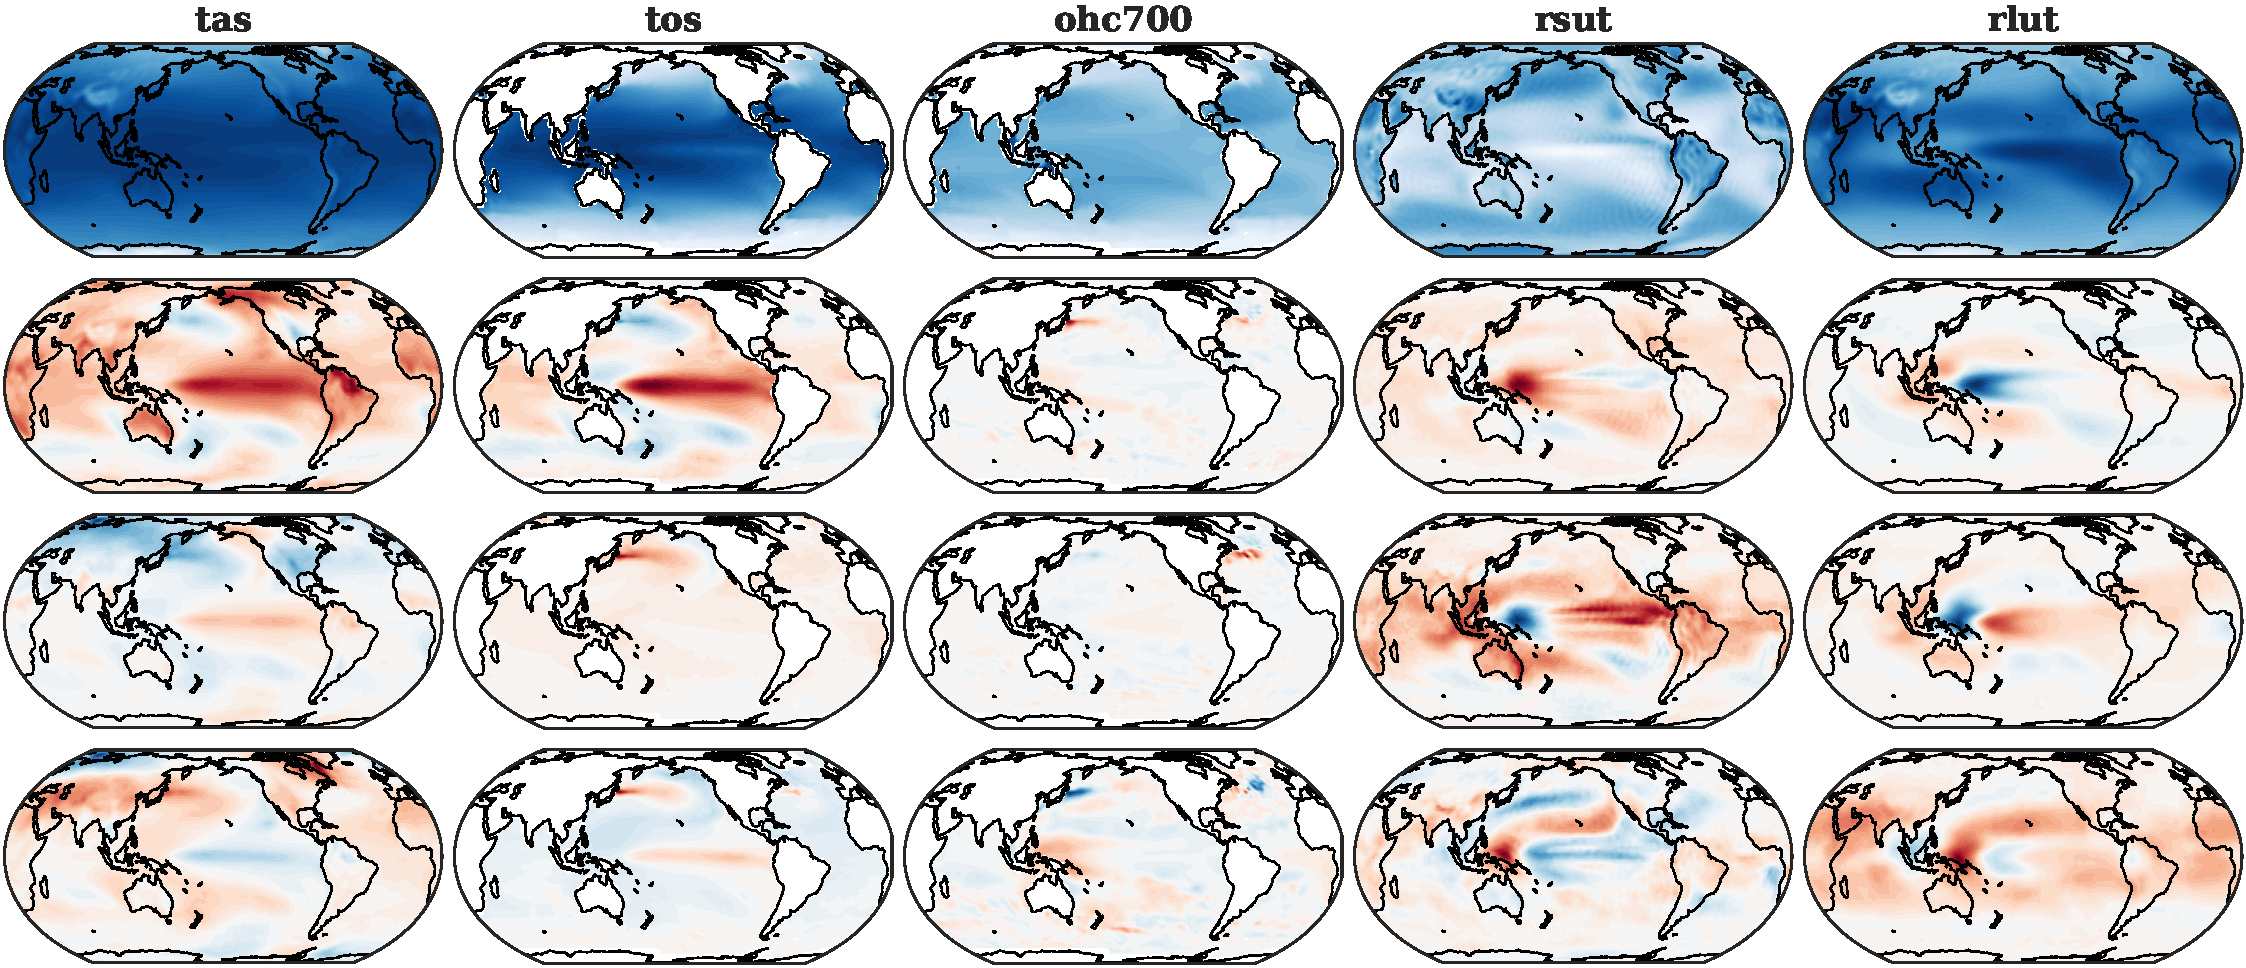
\includegraphics[width=\textwidth]{figures/plots/eofs.pdf}
    \caption{Mean (top) and first three \glspl{EOF} (below) for a selection of fields.}
    \label{fig:eofs-mine}
\end{figure}

\cref{fig:eofs-mine} shows the mean and leading \glspl{EOF} that my code found. All of them look physical (as far as I can judge) and show well-known patterns such as ENSO in TAS/TOS and the Indonesian Throughflow on RSUT/RLUT. The OHC700 field is clearly distinct with less spatial variability. This substantiates its separate treatment in the reduction procedure.

\begin{figure}[h]
    \centering

    \begin{subfigure}[c]{0.3\textwidth}
        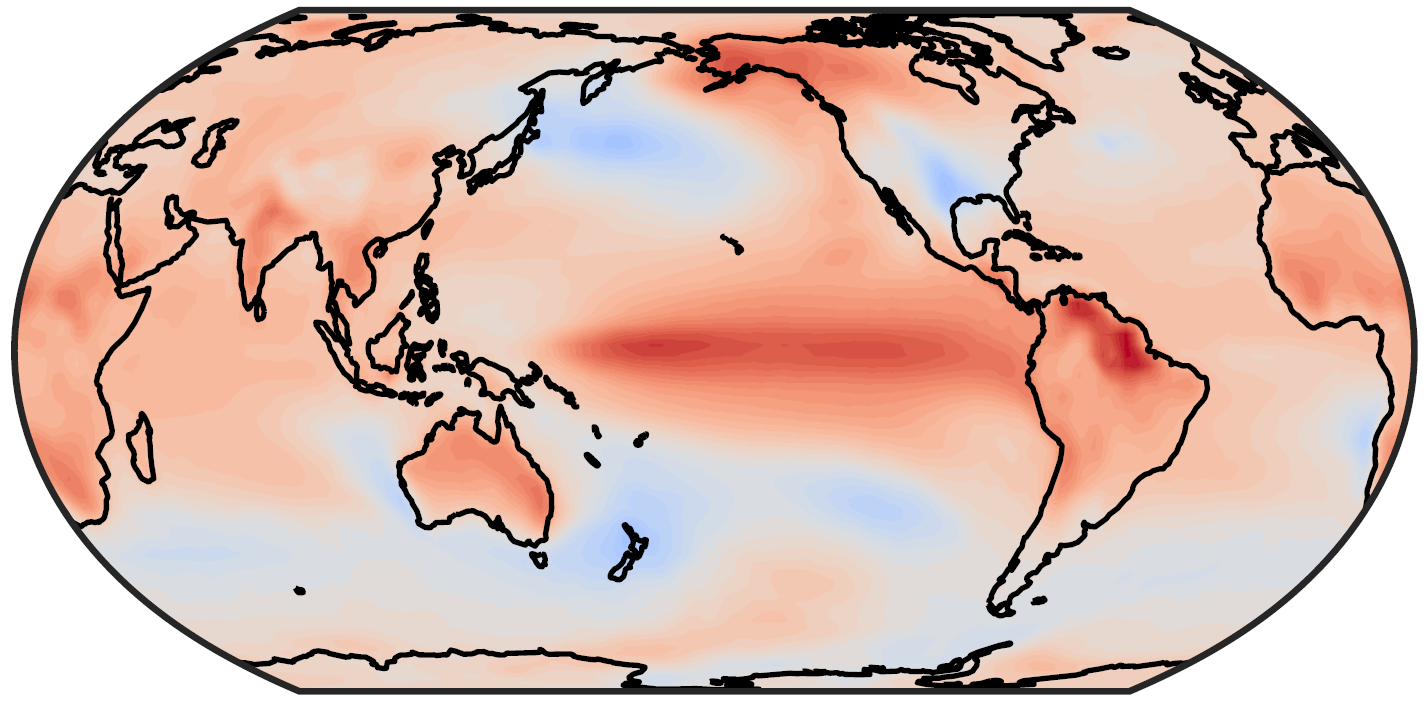
\includegraphics[width=\textwidth]{figures/eoftas_mine.png}
        \subcaption{Mine (CMIP6 MPI)}
        \label{fig:eofs-ph-mine}
     \end{subfigure}
     \hfill
     \begin{subfigure}[c]{0.3\textwidth}
        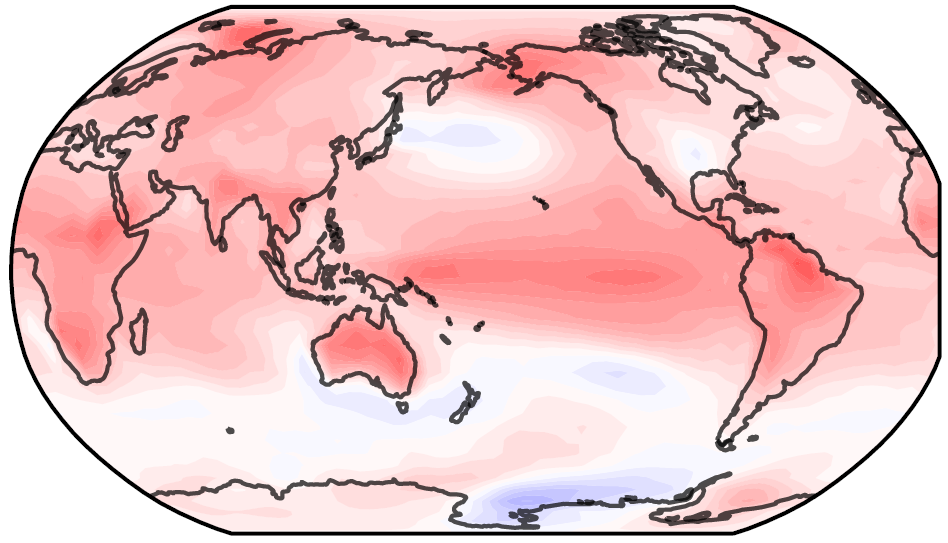
\includegraphics[width=\textwidth]{figures/eoftas_ph17_mpi.png}
        \subcaption{PH17 (CMIP5 MPI)}
     \end{subfigure}
     \hfill
     \begin{subfigure}[c]{0.3\textwidth}
        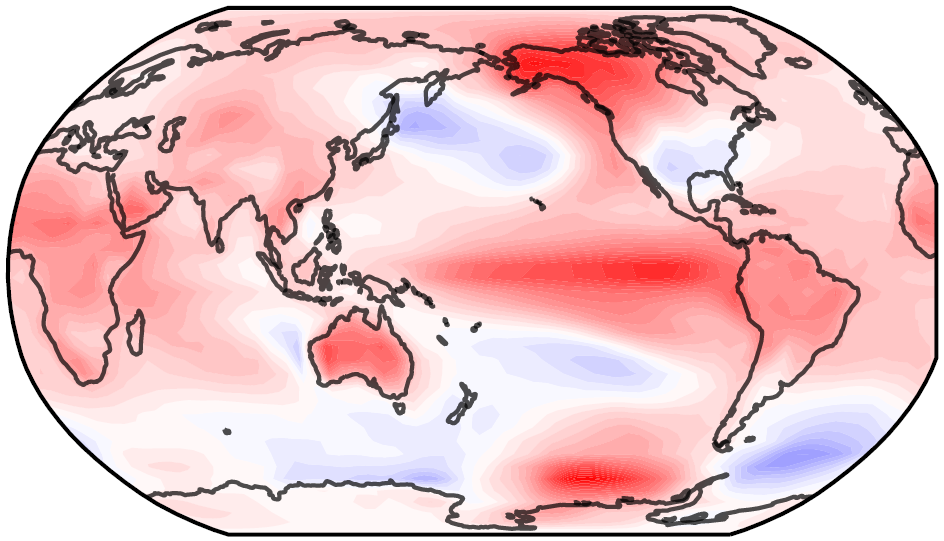
\includegraphics[width=\textwidth]{figures/eoftas_ph17_ccsm.png}
        \subcaption{PH17 (CMIP5 CCSM)}
     \end{subfigure}

    \caption{Leading EOFs for TAS from my and PH17's reconstructions.}
    \label{fig:eofs-ph}
\end{figure}

We can compare the leading \gls{EOF} of TAS (first column, second row in \cref{fig:eofs-mine}, also \cref{fig:eofs-ph-mine}) to those found by PH17 in \cref{fig:eofs-ph}. Their \glspl{EOF} are derived from CMIP5 \emph{past1000} outputs of the CCSM and MPI models while mine comes from the CMIP6 \emph{past2k} experiment of the MPI model. The patterns are generally similar: a pronounced warm pattern in the tropical Pacific is flanked by colder regions; hot Australian and North American continents. The Southern Ocean and South America regions show more similarity between the MPI models, but cool region in the North Pacific is smaller in the CMIP5 MPI version. Still, the \glspl{EOF} are similar enough for us to conclude that the choice of training data has little effect on the TAS reconstructions.



\subsection{LIM for forecasting}
\label{subsec:setup-lim}

The \gls{LIM} is an efficient forecast model that makes online \gls{DA} computationally feasible. The forecast allows information to be propagated through time, particularly by inclusion of OHC700, which acts as dynamic memory to inform low-frequency variability. In addition, the cheap forecasting enables large ensembles: forecasting my 100 ensemble members for a year takes less than 1 s.

A \gls{LIM} can represent a linear system of the form
\begin{align*}
    \dv{\vb{x}}{t} = \vb{L}\vb{x} + \vb*{\xi},
\end{align*}
where $\vb{L} \in \mathbb{R}^{N_x \times N_x}$ is a linear operator and $\xi \sim N(0, \vb{Q}/dt)$ is additive Gaussian noise. In my case, the state dimension is $N_x = 50$. The deterministic forecast equation is then~\parencite{Penland1995}
\begin{align*}
    \vu{x}_{k+1} = \exp (\vb{L} \, \Delta t) \, \vb{x}_k  = \vb{G} \vb{x}_k ,
\end{align*}
where $\vb{G} \in \mathbb{R}^{N_x \times N_x}$ is the linear forecast operator. For probabilistic ensemble forecasts, we can use the two-step stochastic integration scheme proposed by \textcite{Penland1994}:
\begin{align}
    \label{eq:stoch-forecast}
    \vb{x'}(t+\delta t) &= \vb{x'}(t) + \vb{L}\vb{x'}(t) \, \delta t + \vu{Q} \sqrt{\vb{\Lambda}\delta t} \mathcal{R},
    \\
    \vb{x}(t + \delta t / 2) &= \left[\vb{x'}(t) + \vb{x'}(t+\delta t)\right] / 2,
\end{align}
where $\vu{Q}$ and $\vb{\Lambda}$ come from the eigendecomposition $\vb{Q} = \vu{Q} \vb{\Lambda}\vu{Q}^{-1}$ of the noise covariance matrix and $\mathcal{R}$ is a vector of random numbers drawn from a standard normal distribution. The integration timestep $\delta t$ must be chosen much smaller than the corresponding deterministic timestep $\Delta t$. PH21 used $\delta t \approx \qty{6}{h}$, which requires 1440 integration steps over a period of $\Delta t = \qty{1}{year}$; I used the same $\delta t$.

The system dynamics $\vb{L}$ and $\vb{G}$ as well as the noise covariance $\vb{Q}$ can be determined from data. The procedure is based on the zero-lag and $\tau$-lag covariance matrices:
\begin{align*}
    \vb{C}(0) = \langle \vb{x}(t) \vb{x}^\transpose*(t) \rangle \qquad \mathrm{and} \qquad \vb{C}(\tau) = \langle \vb{x}(t+\tau) \vb{x}^\transpose*(t) \rangle,
\end{align*}
where $\langle \cdot \rangle$ denotes the time average. In my case, the average is over 1848 timesteps (one year is removed by the split-year annual average, another by the 1-year lag). The forecast operator is then recovered as
\begin{align*}
    \vb{G} = \vb{C}(\tau) \vb{C}(0)^{-1}.
\end{align*}
This reveals $\vb{G}$ to be the sensitivity between the states of two $\tau$-lagged timesteps, normalized by the state covariance. The linear operator $\vb{L}$ required for stochastic integration is then found as
\begin{align*}
    \vb{L} = \frac{\ln\vb{G}}{\tau}.
\end{align*}
The logarithm is preferably evaluated by eigendecomposition of $\vb{G}$. Finally, we can find the noise covariance matrix as
\begin{align}
    \label{eq:noise-cov}
    \vb{Q} = - \left( \vb{L} \vb{C}(0) + \vb{C}(0) \vb{L} \right).
\end{align}
While covariance matrices are positive semi-definite, the $\vb{Q}$ found here may have spurious negative eigenvalues as a result of a short training period or significant non-linear dynamics~\parencite{Penland1994}. We can remove these negative eigenvalues by eigendecomposition of $\vb{Q}$, but have to rescale the remaining ones to retain the total variance.



\subsection{EnSRF for data assimilation}
\label{subsec:setup-ensrf}

The ensemble forecast from the \gls{LIM} requires a \gls{DA} scheme that is compatible with ensemble priors. For simplicity, I use the \gls{EnSRF}~\parencite{Whitaker2002} also employed in PH17, while PH21 used an ensemble transform Kalman filter. Nonetheless, the results should be similar if not identical between the two. I did not have time to implement covariance localization and calibrate my filter through inflation or additive noise.

The \gls{EnSRF} works on the assumption that observations are independent so that Bayes' rule can be applied sequentially. First, the ensemble is converted into perturbations
\begin{align*}
    \vb{X} = \mqty[ \vb{x}^{1} - \vu{x} &  \vb{x}^{2} - \vu{x} & \ldots &  \vb{x}^{N_e} - \vu{x} ],
\end{align*}
where $\vb{x}^i$ are the ensemble priors (column vectors) and $\vu{x}$ is their mean. In my case, the number of ensemble members is $N_e = 100$. We then define the ensemble prior of the observations
\begin{align*}
    \vb{Z} = \vb{H} \vb{X},
\end{align*}
which allows us to efficiently compute the variance of the observation forecast as
\begin{align*}
    \hat{\sigma}_p^2 = \frac{\vb{Z} \vb{Z}^\transpose}{N_e-1}.
\end{align*}
The analysis ensemble perturbations are then
\begin{align*}
    \vb{X}^a = \vb{X} \left( \vb{I}_{N_e} - \alpha \frac{\vb{Z} \vb{Z}^\transpose*}{(N_e-1)(\hat{\sigma}_p^2 + \sigma_o^2)} \right),
\end{align*}
where $\sigma_o^2$ is the observation variance. Notice that the analysis perturbations must be in the span of the prior perturbations. The scalar $\alpha$ such that the analysis covariance is correct is found as
\begin{align*}
    \alpha = \left( 1 + \sqrt{\frac{\sigma_o^2}{\hat{\sigma}_p^2 + \sigma_o^2}} \right)^{-1}.
\end{align*}
Next, we compute the analysis ensemble mean as
\begin{align*}
    \vu{x}^a = \vu{x} + \frac{\vb{X}\vb{Z}^\transpose}{(N_e-1)(\hat{\sigma}_p^2 + \sigma_o^2)} \left( y - \vb{H} \vu{x} \right).
\end{align*}
Finally, we combine mean and perturbations to form the posterior ensemble
\begin{align*}
    \left(\vb{x}^i\right)^a = \vu{x}^a + \vb{X}^a_i,
\end{align*}
which is the initial condition for the next forecast of the \gls{LIM}.




\subsection{Setup for cycling data assimilation}

For this project, I only reconstruct the 200-year period of 850-1050 CE due to time constraints. I fitted the physical--reduced space mapper on the Casper cluster, which produced the training dataset for the \gls{LIM} in the process. The remaining steps (fitting the \gls{LIM}, running the reconstruction, and analyzing the results) were performed on Greg's \texttt{enkf} server.

\begin{figure}[h]
    \centering
    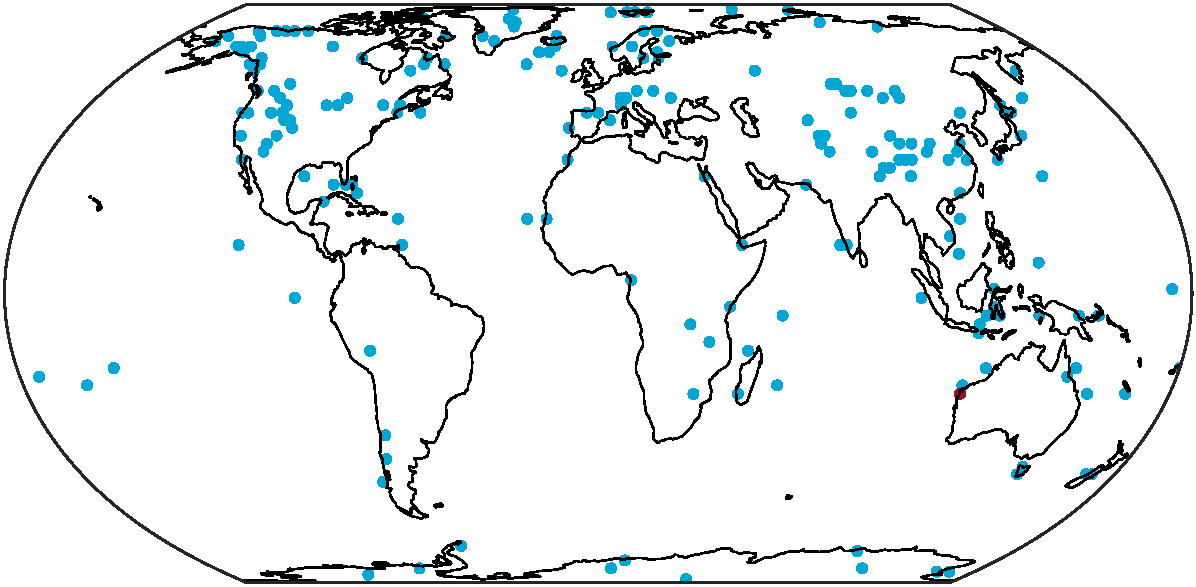
\includegraphics[width=0.5\textwidth]{figures/plots/obs_locations.pdf}
    \caption{Pseudo-observation locations, a sample of 200 locations from the Pages2k proxy dataset. Observation location \#1 at the coast of Australia is marked in red.}
    \label{fig:obs-locs}
\end{figure}

My ensemble has 100 members, which are initialized from a random draw of 100 years from the training dataset. My pseudo-observations come from annual averages of the CMIP6 \emph{past1000} output of the MRI-ESM2-0 model. Despite the similar name, this model is has no shared lineage with the MPI-ESM1-2-LR model of the training dataset. Drawing them from a different model than the training data should lead to a more challenging testbed for my \gls{DA} system. The observations are surface air temperatures from locations of the Pages2k proxies~\parencite{PAGESConsortium2017}, which is the real dataset used by PH21. I drew a random sample of 200 locations (the same ones for every year of the reconstruction), which is roughly the average of the number of proxies assimilated per year in PH21. The 200 locations are shown in \cref{fig:obs-locs}. While there are few observations over the oceans, their coverage is global otherwise. The pseudo-observations were perturbed by Gaussian noise with $\sigma_o^2 = \qty{1}{K^2}$, which is also the observation variance used in the \gls{EnSRF}.




\section{LIM results}

We consider \gls{LIM}-only results first to assess the forecast behavior.

\subsection{Fitted dynamics and noise covariance}

\begin{figure}[h]
    \centering
    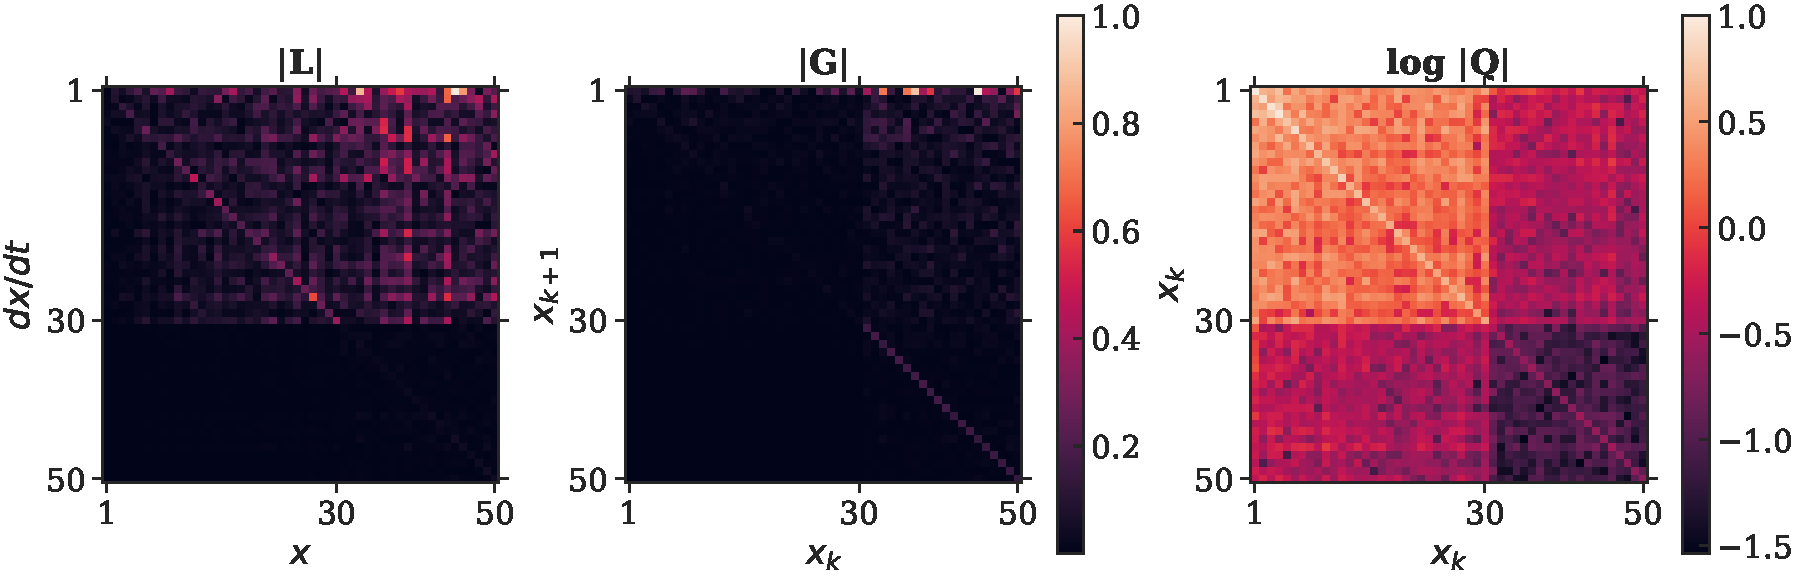
\includegraphics{figures/plots/lim_matrices.pdf}
    \caption{System dynamics matrices $\vb{L}, \vb{G}$ and noise covariance matrix $\vb{Q}$.}
    \label{fig:lim-matrices}
\end{figure}

\cref{fig:lim-matrices} shows the system dynamics matrices $\vb{L}, \vb{G}$ and noise covariance matrix $\vb{Q}$ of the LIM. A block structure is discernible in all three. The blocks correspond to the 30-element joint EOF of fast fields (1-30) and the 20-element EOF of OHC700 (31-50) (cf. \cref{subsec:setup-dimred}). This separation is particularly clear in $|\vb{L}|$, for which the derivatives of the slow OHC700 are the smallest. On the other hand, the OHC700 field does significantly influence the leading mode of the joint EOF as seen by the bright elements in the first rows of $|\vb{L}|$ and $|\vb{G}|$. Additionally, each element affects itself significantly during the forecast as indicated by the bright diagonal. Blocks are also visible in the system noise covariance matrix $\vb{Q}$, which has large covariances between the fast fields, smaller between the fast fields and OHC700, and the smallest between modes of OHC700.

I also checked the eigenvalues of $\vb{L}$, which determine the forecast stability. Unexpectedly, $\vb{L}$ is a complex matrix even though the system state $\vb{x}$ is real. $\vb{L}$ is determined from the eigendecomposition $\vb{G} = \vu{G} \Lambda\vu{G}^{-1}$ as $\vb{L} = \vu{G} \left(\tau^{-1}\log\vb{\Lambda}\right)\vu{G}^{-1}$. While $\vb{G}$ is real, $\vu{G} \Lambda\vu{G}^{-1}$ has imaginary components of $\mathcal{O}(10^{-18})$--$\mathcal{O}(10^{-14})$. Due to $\log\vb{\Lambda}$, these small differences are amplified such that the imaginary components of $\vb{L}$ are of the same magnitude as the real ones. By \cref{eq:noise-cov}, this then also propagates to the covariance matrix $\vb{Q}$, which is Hermitian instead of symmetric. Judging from the PH21 code, they ran into the same problem. I handled it as they did: keep $\vb{L}$ and $\vb{Q}$ complex and take the real part of the forecast from \cref{eq:stoch-forecast}.

\begin{figure}[h]
    \centering
    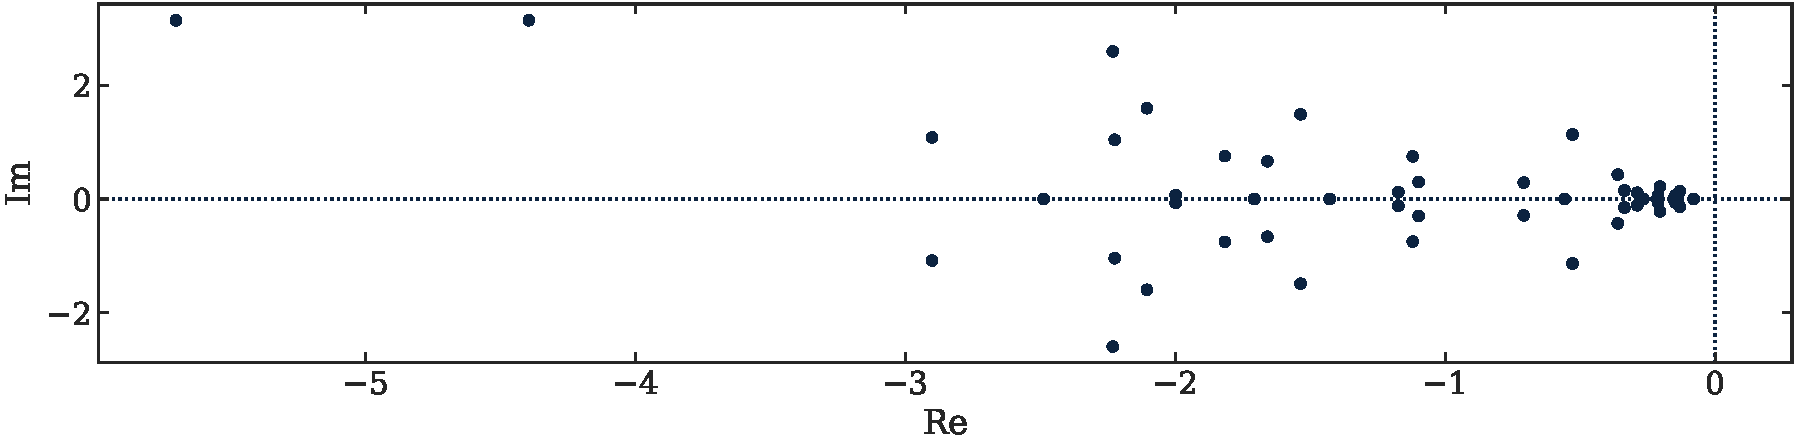
\includegraphics{figures/plots/lim_eigs.pdf}
    \caption{Eigenvalues of $\vb{L}$, which govern the system's stability.}
    \label{fig:lim-eigs}
\end{figure}
\cref{fig:lim-eigs} shows the eigenvalues of $\vb{L}$. Since $\vb{L}$ is complex, not all eigenvalues appear in complex conjugate pairs as one would expect, but most do. More important is the negative real part of all eigenvalues, which makes the LIM forecast stable and decay to zero for long lead times (this is by construction). Most modes have an ocscillatory component, but their frequencies vary.



\subsection{Free run}

\begin{figure}[h]
    \centering
    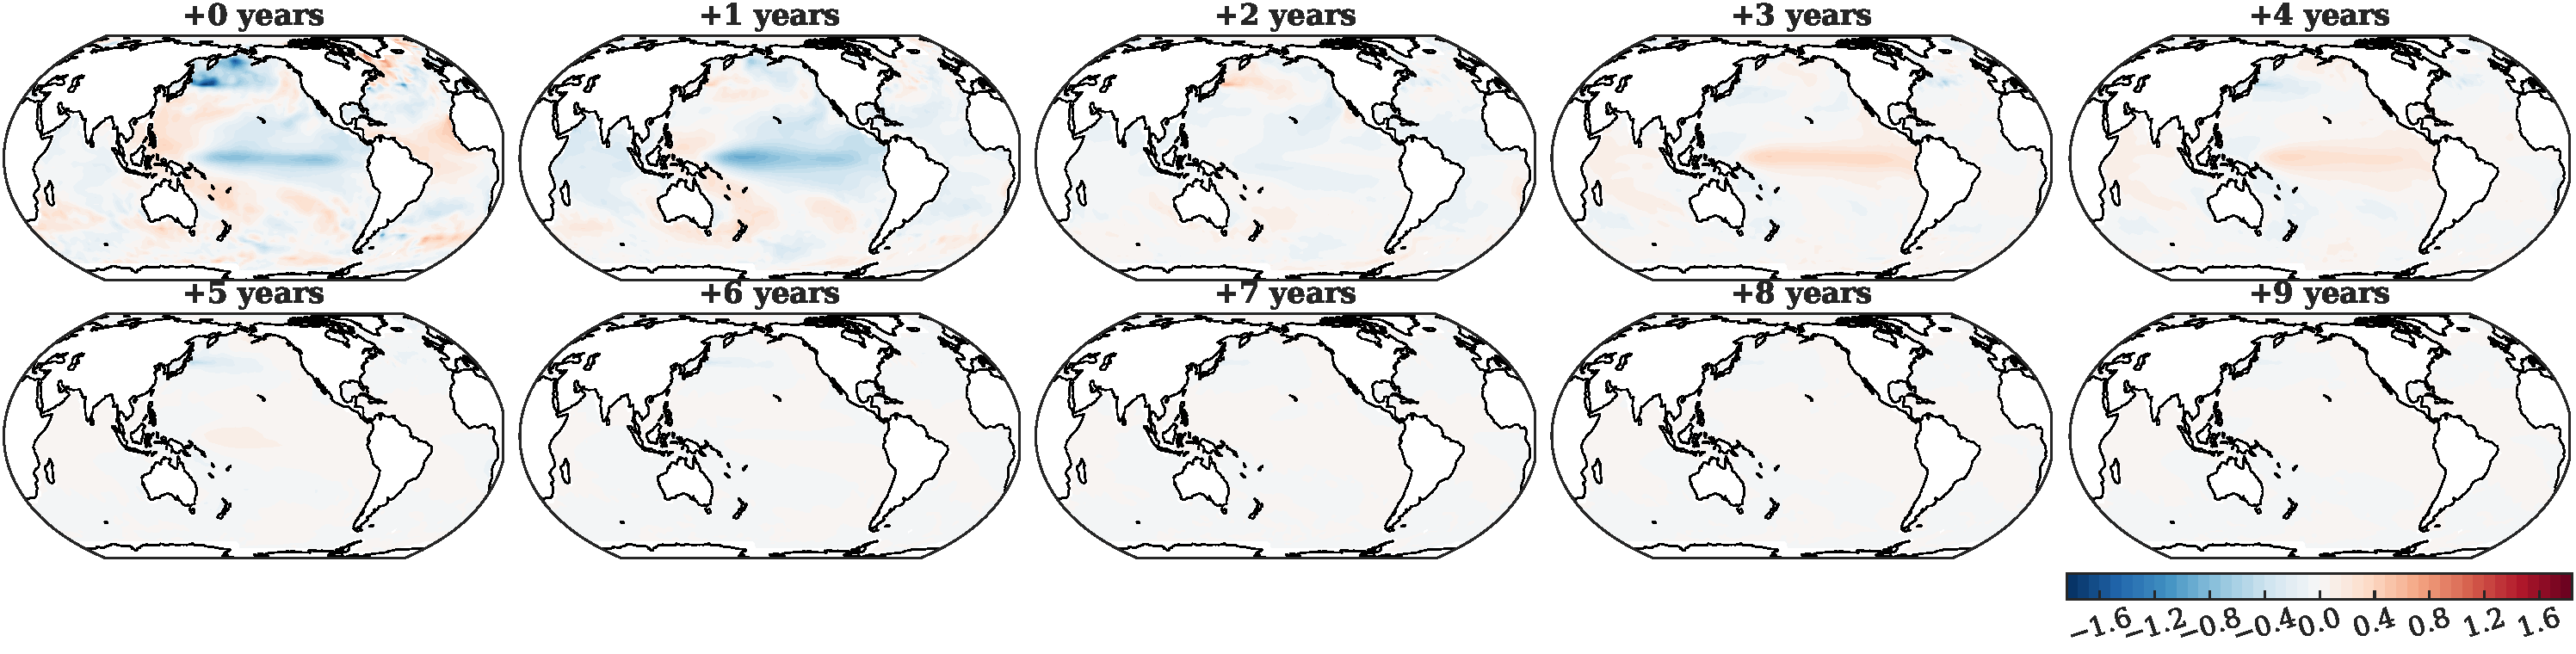
\includegraphics{figures/plots/fc_free_tos_anomaly.pdf}
    \caption{Free-run forecast for sea surface temperature.}
    \label{fig:freerun-tas}
\end{figure}

Assessing free runs of the LIM without DA can tell us about its forecast skill. \cref{fig:freerun-tas} shows an example of the sea surface temperature (TOS) over a 9-year forecast. The initial condition features a La Niña pattern of cold temperatures in the Pacific, which persists over the first year. In years three and four, the warm anomaly associated with El Niño is visible. The pattern observed is captured by the leading EOF of the TOS field (cf. \cref{fig:eofs-mine}) and is an example of the oscillatory eigenmodes seen in the last subsection. Beyond five years, the forecast decays to zero. A similar behavior is present in the other fields.


\begin{figure}[h]
    \centering

    \begin{subfigure}[c]{0.77\textwidth}
        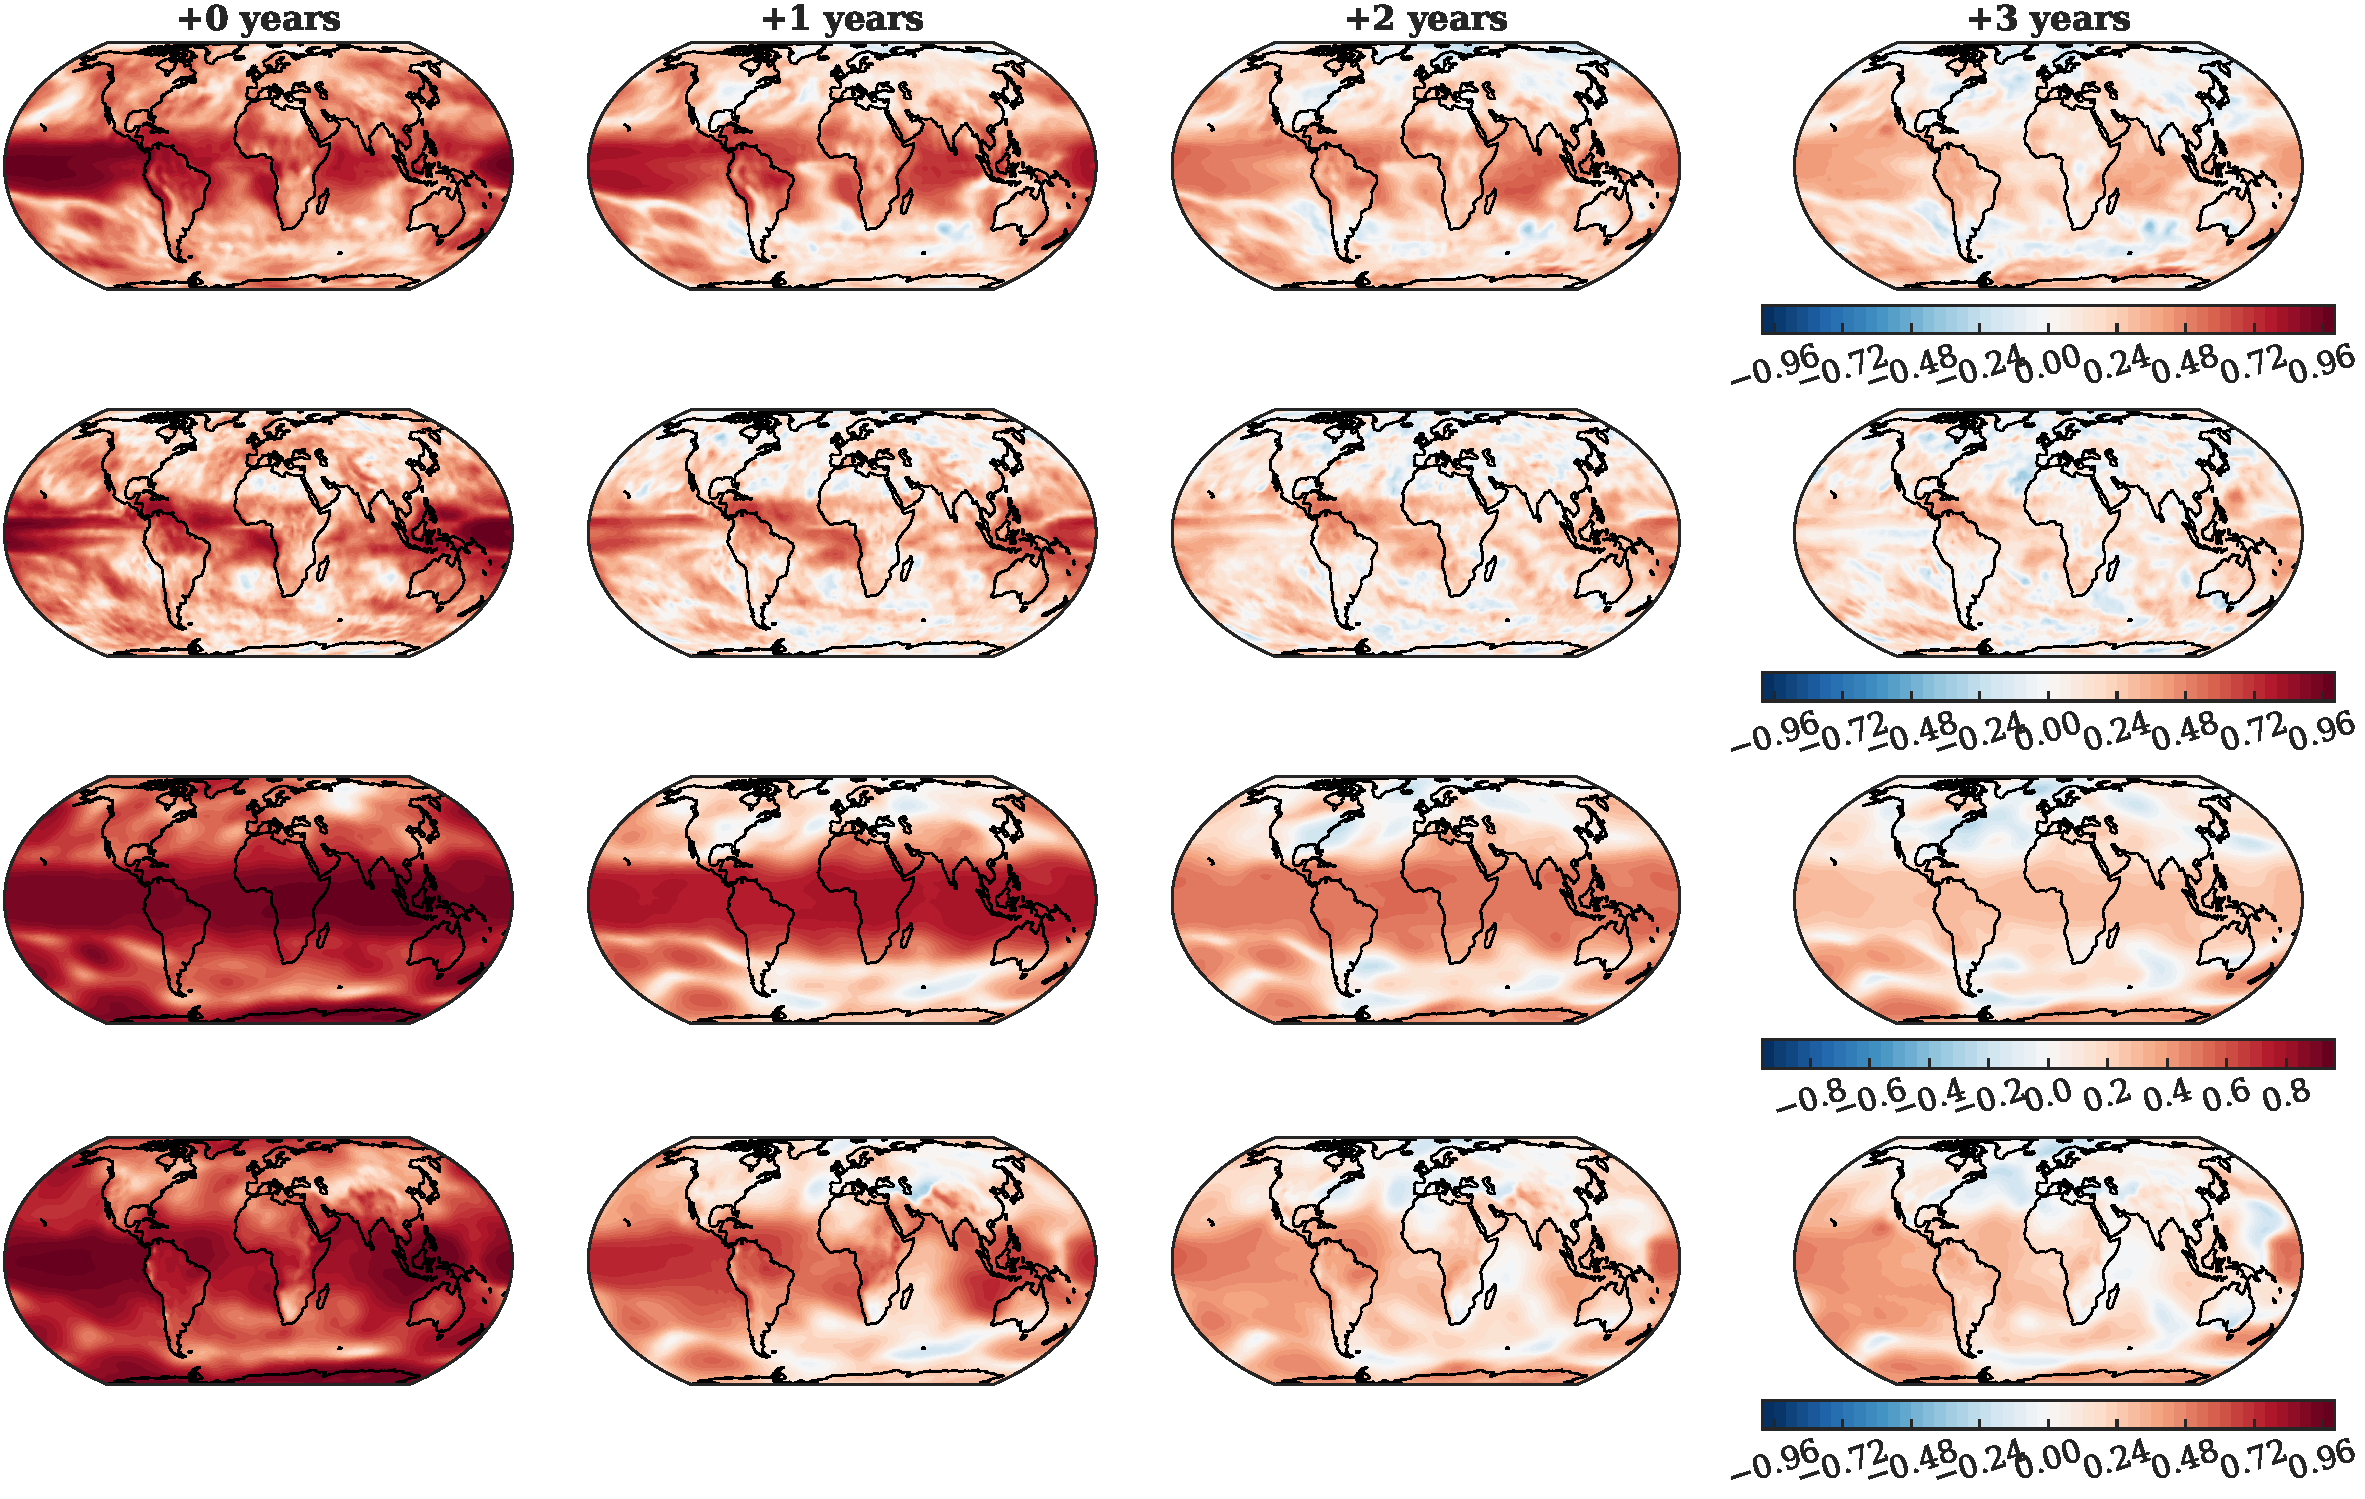
\includegraphics[width=\textwidth]{figures/plots/corr_spatial.pdf}
        \subcaption{Mine (CMIP6 MPI)}
        \label{fig:corr-spatial-mine}
    \end{subfigure}
    \hfill
    \begin{subfigure}[c]{0.22\textwidth}
        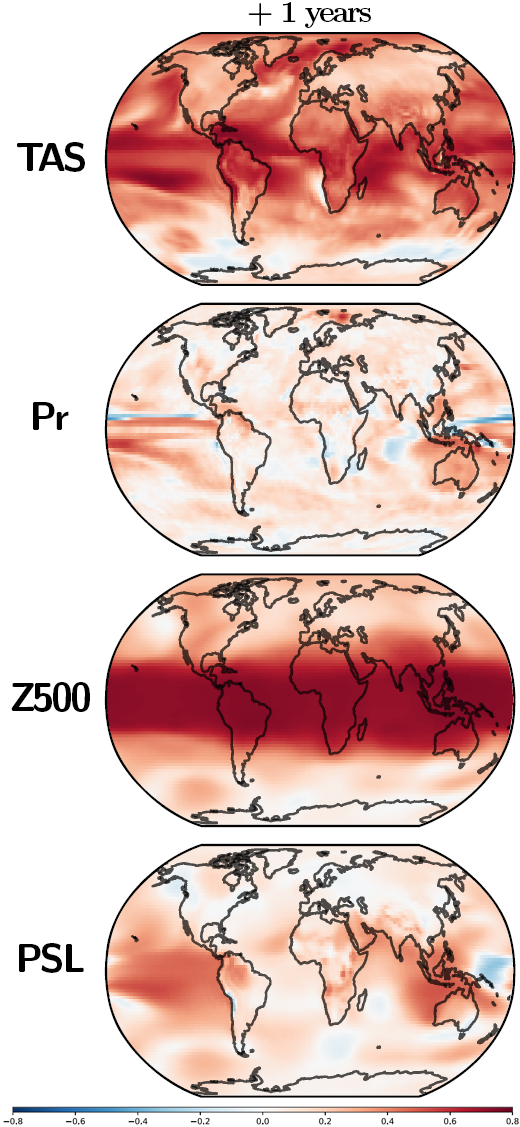
\includegraphics[width=\textwidth]{figures/corr_spatial_ph20.png}
        \subcaption{PH20 (CMIP5 MPI)}
        \label{fig:corr-spatial-ph}
     \end{subfigure}
    \caption{Spatial correlations between the LIM forecast and its training data, averaged over 100 cases. The correlations from PH20 are for a 1-year lead time.}
    \label{fig:corr-spatial}
\end{figure}

\cref{fig:corr-spatial-mine} shows the spatial correlations of LIM forecast and training data over different lead times, averaged over 100 cases. The fields shown are surface air temperature, precipitation, 500 hPa geopotential height, and sea-level pressure. The initial condition is not perfectly correlated since some information was lost in the dimensionality reduction. At a 1-year lead time, the correlation for Z500, PSL, and TAS is still high, particularly in the tropics. The precipitation skill is lower both in the initial condition and after 1 year, possibly because it does not have much shared variability and its information is therefore lost in the joint EOF. Beyond 2--3 years, the LIM does not have much skill on any field.

We can also compare the spatial correlations after 1 year to those found by PH20. The global pattern is very similar, particularly for TAS and Z500. However, the TAS field of PH20 has higher correlations in the Northern hemisphere. The correlation of my PSL is more consistently high across all longitudes, particularly above the Atlantic and Africa. Interestingly, mine has large positive correlations over the Indonesian Throughflow (northeast of Australia) while PH20 have large negative correlations. Finally, the precipitation fields in my forecast have higher correlations above the Atlantic, but the streaks over the Pacific are present in both. In general, we can conclude that the 1-year forecasts have similarly high correlations and any differences can likely be attributed to the different training datasets.



\section{DA results}

To assess the quality of the DA results, we compare them against the same dataset from which the observations are drawn, but without the noise. This choice of verification dataset tells us about the skill of the DA system as a whole rather than just the forecasting model, which was compared to its training dataset in the last section. All spatial means in this section are area-weighted by $\sqrt{\cos\phi}$.



\subsection{Sanity check}
First, I checked if my \gls{EnSRF} includes gross errors. In particular, I compared prior and posterior variances to see if the variance always decreases; they do. The variances of atmospheric fields and sea surface temperature are reduced by \qtyrange{50}{60}{\percent}. Interestingly, the largest reduction is seen not in TAS (\qty{56}{\percent}), which is the observed field, but in ZG500 (\qty{60}{\percent}). The uncertainty of OHC700 is reduced the least (\qty{21}{\percent}). For the observed TAS field, the observation variance is $\sigma_o^2 = \qty{1}{K^2}$ as described above, and the mean prior ensemble variance is $\hat\sigma_p^2 = \qty{0.09}{K^2}$. The mean posterior ensemble variance is $\qty{0.04}{K^2}$.

\begin{figure}[h]
    \centering

    \begin{subfigure}[c]{\textwidth}
        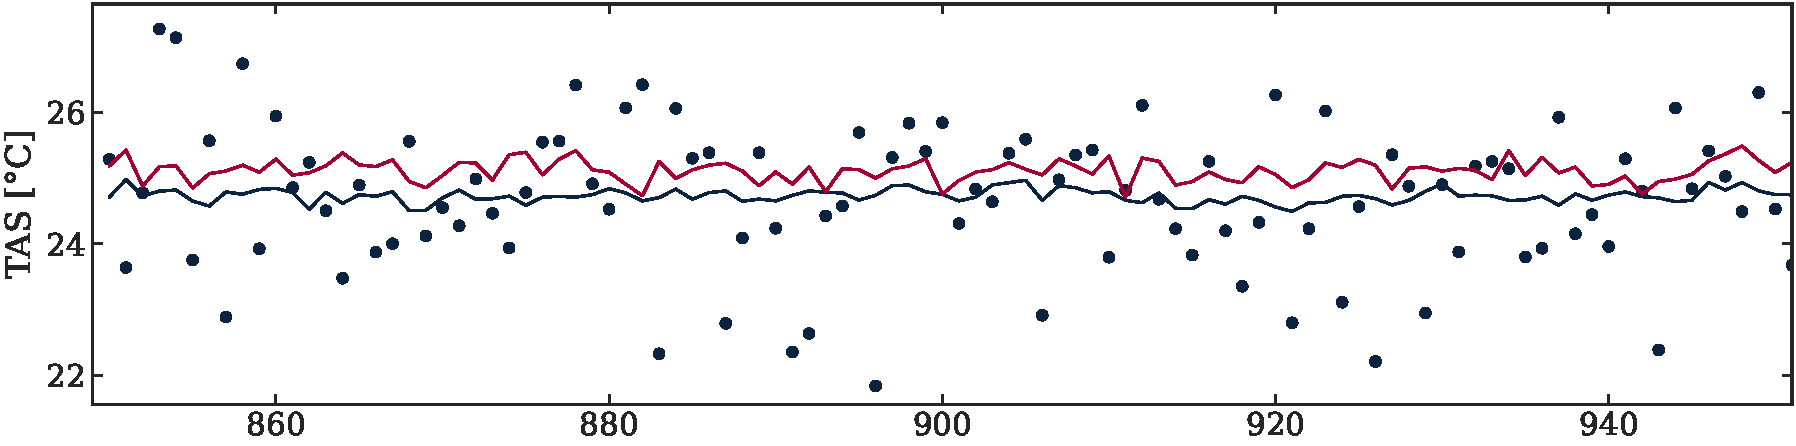
\includegraphics[width=\textwidth]{figures/plots/tas_obs_vs_reconstruction.pdf}
        \subcaption{At observation location \#1}
        \label{fig:tas-obs-reconstruction}
    \end{subfigure}
    
    \bigskip
    
    \begin{subfigure}[c]{\textwidth}
        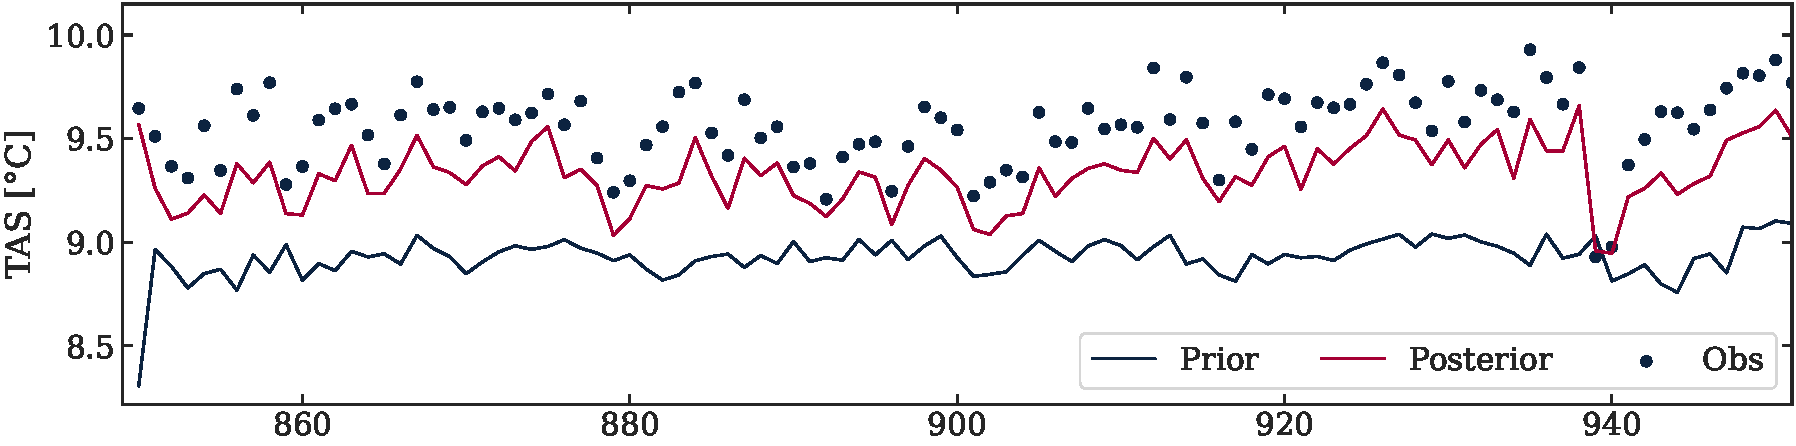
\includegraphics[width=\textwidth]{figures/plots/tas_obs_vs_reconstruction_mean.pdf}
        \subcaption{Mean over all observation locations}
        \label{fig:tas-obs-reconstruction-mean}
     \end{subfigure}
    
    \bigskip
    
    \begin{subfigure}[c]{\textwidth}
        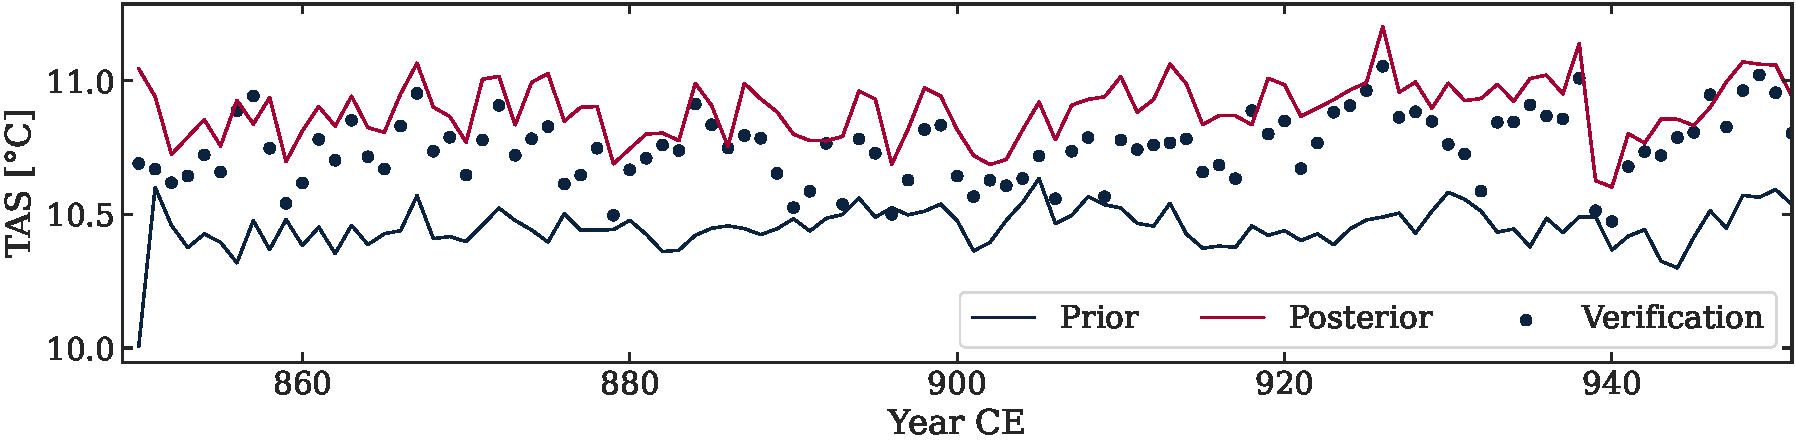
\includegraphics[width=\textwidth]{figures/plots/tas_obs_vs_reconstruction_mean_all.pdf}
        \subcaption{Global mean}
        \label{fig:tas-obs-reconstruction-mean-all}
     \end{subfigure}

    \caption{Prior, posterior, and observations/verification for surface air temperature over a 100-year period. In the mean, the posterior is always between prior and observation, but not necessarily at each location.}
\end{figure}

Another principle of the \gls{EnSRF} is that, for a single observation, the analysis at that location is always between the prior and the observation since it constitutes a weighted average. This is not the case when multiple observations are assimilated (\cref{fig:tas-obs-reconstruction}). However, in the mean over all 200 observation locations, the posterior is indeed bounded by the prior and observations (\cref{fig:tas-obs-reconstruction-mean}). Notice that the temperatures at observation location \#1 are \qty{15}{\K} warmer than in the mean over all observation locations; the reason is that this observation originates from the Australian coast (red dot in \cref{fig:obs-locs}).

An interesting point to note is that the observations are consistently warmer than the prior at the observation locations (\cref{fig:tas-obs-reconstruction-mean}), even though the verification dataset (same as observations but global coverage and noise-free) is closer to the prior in the global mean (\cref{fig:tas-obs-reconstruction-mean-all}). This may indicate that the 200 Pages2k locations I randomly sample are biased towards warm regions. As a result, the posterior is also consistenly warmer than the prior, which distorts the global mean surface temperature. Note that I assimilated observations as absolute temperature, not anomalies, which may be a source of bias between observations and forecast. Still, this does not explain why the verification is more similar to the prior.




\subsection{Reconstruction}

\begin{figure}[h]
    \centering
    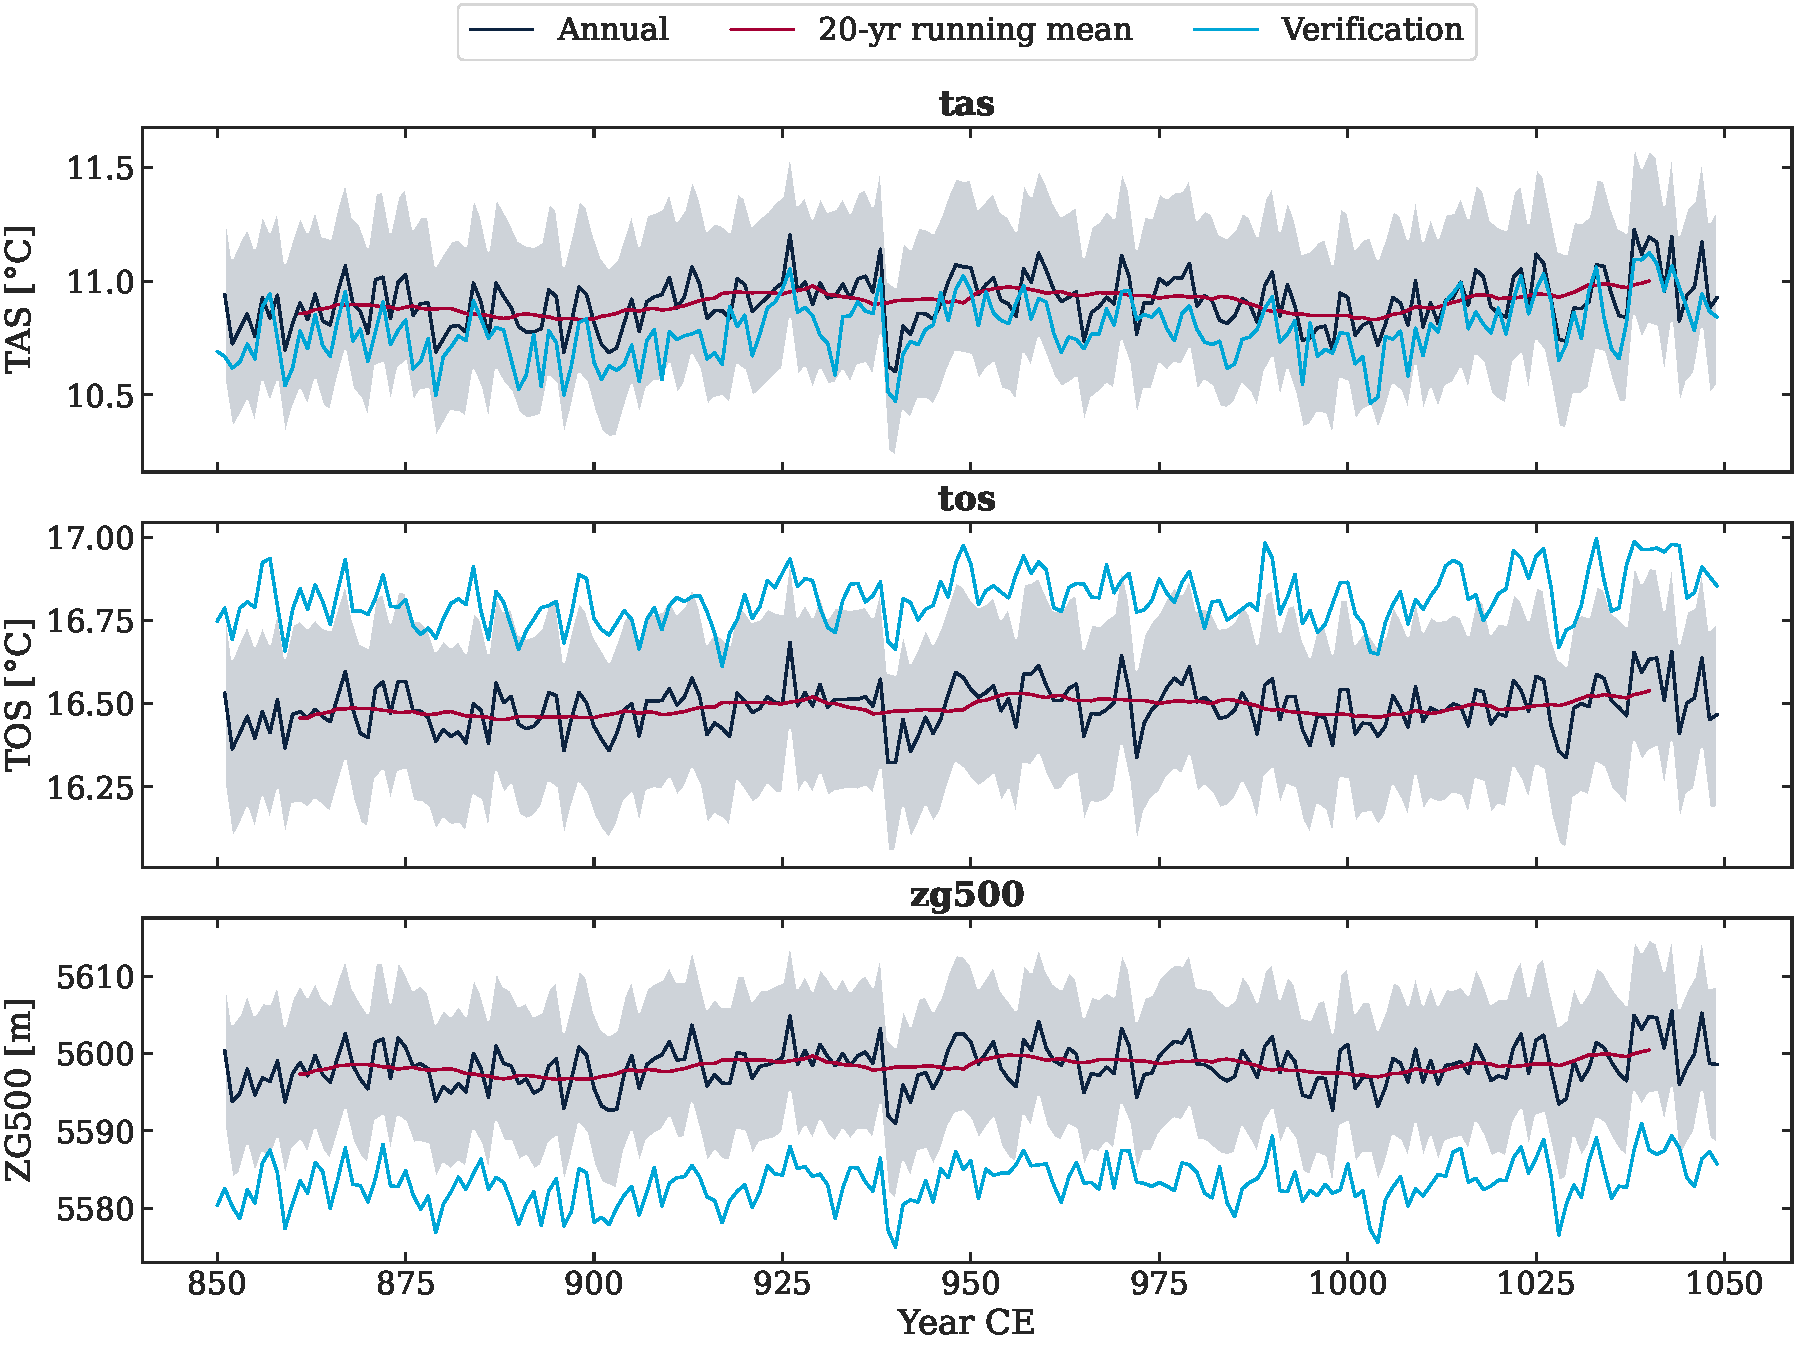
\includegraphics{figures/plots/field_reconstruction_mean.pdf}
    \caption{Global mean reconstructions. Gray shading denotes the 95\% confidence interval.}
    \label{fig:reconstruction-mean}
\end{figure}

\cref{fig:reconstruction-mean} shows reconstructions of the global means of TAS, TOS, and ZG500. In the 20-year running mean, the surface air temperatures are around \qty{11.8}{\celsius} while the sea surface temperatures are much warmer at \qty{16.5}{\celsius}; these are realistic values. The 500 hPa geopotential height is also in a physical range. Over the 200-year period, the three fields are essentially stationary.

I also compared the fields to the verification dataset in \cref{fig:reconstruction-mean}. For TAS, the verification is slightly lower than the reconstruction, as we already saw in \cref{fig:tas-obs-reconstruction-mean-all}, but well within the 95\% confidence interval. However, this is not the case for TOS and ZG500: the verification is outside this interval for almost every year of the 200-year period. The difference appears to be an almost constant offset, which is similar to what we saw for TAS prior and obsevations in \cref{fig:tas-obs-reconstruction-mean}. This suggests that the bias in TAS observations appears amplified in the other fields.


\begin{figure}[h]
    \centering
    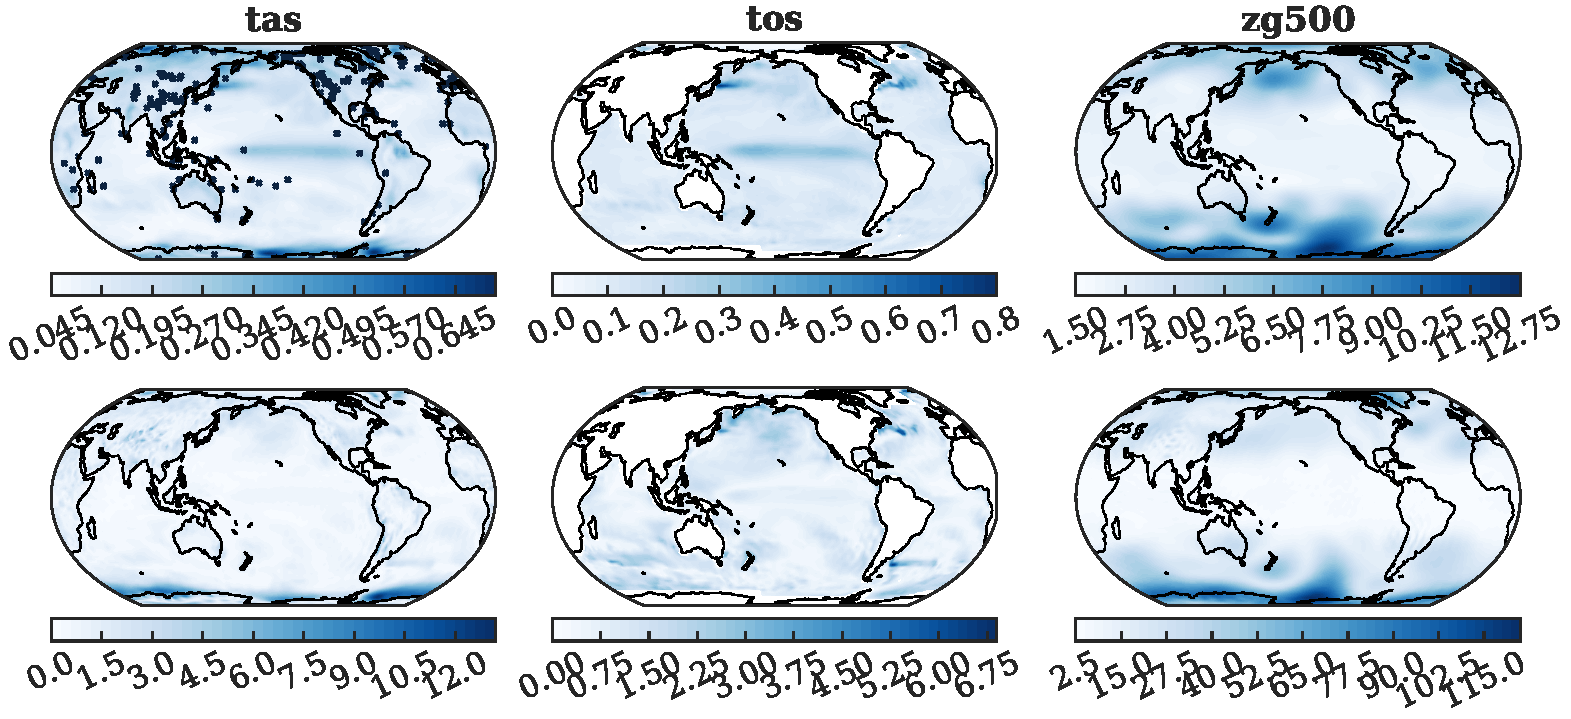
\includegraphics{figures/plots/var_vs_sqerr.pdf}
    \caption{Spatial distribution of ensemble standard deviation (top row) and root-mean-squared error (bottom row). The ensemble grossly underestimates the spread. Observation locations are marked in the TAS plot.}
    \label{fig:var-vs-sqerr}
\end{figure}

In addition to observation bias, there is another reasonable explanation for why the verification falls outside the posterior confidence interval: the ensemble is underdispersive. As mentioned earlier, the estimated prior variance is $\hat\sigma_p^2 = \qty{0.09}{K^2}$, which is very small for a 1-year forecast and much smaller than the observation covariance of $\sigma_o^2 = \qty{1}{K^2}$. This explanation is also supported by the comparison of ensemble posterior standard deviation and the root-mean-squared error of the posterior mean, averaged over the 200-year period (\cref{fig:var-vs-sqerr}). The ensemble spread underestimates the error by an order of magnitude. The spatial distribution is also different, although both are worse in polar regions, likely due to the latitude-weighting during the dimensionality reduction. There is also no clear relation to the observation locations (shown in the upper TAS plot), where one may expect lower errors. This is particularly true for Antarctica, which should be constrained by ten observations

There are two solutions to increasing the ensemble spread. Ideally, the stochastic LIM forecast would introduce the spread based on the noise learned from the training data. After checking that the noise covariance matrix $\vb{Q}$ is indeed correct, it could be calibrated to match variance and squared error. This is similar to the second option, which is calibration of the \gls{EnSRF} through additive noise or inflation. I believe that improving the LIM would be the more natural solution since the noise covariance matrix allows direct control of the ensemble spread.




\printbibliography


\end{document}
